\documentclass[]{article}
\usepackage{lmodern}
\usepackage{amssymb,amsmath}
\usepackage{ifxetex,ifluatex}
\usepackage{fixltx2e} % provides \textsubscript
\ifnum 0\ifxetex 1\fi\ifluatex 1\fi=0 % if pdftex
  \usepackage[T1]{fontenc}
  \usepackage[utf8]{inputenc}
\else % if luatex or xelatex
  \ifxetex
    \usepackage{mathspec}
  \else
    \usepackage{fontspec}
  \fi
  \defaultfontfeatures{Ligatures=TeX,Scale=MatchLowercase}
\fi
% use upquote if available, for straight quotes in verbatim environments
\IfFileExists{upquote.sty}{\usepackage{upquote}}{}
% use microtype if available
\IfFileExists{microtype.sty}{%
\usepackage{microtype}
\UseMicrotypeSet[protrusion]{basicmath} % disable protrusion for tt fonts
}{}
\usepackage[margin=1in]{geometry}
\usepackage{hyperref}
\hypersetup{unicode=true,
            pdftitle={Review of R/RStudio and EDA},
            pdfborder={0 0 0},
            breaklinks=true}
\urlstyle{same}  % don't use monospace font for urls
\usepackage{color}
\usepackage{fancyvrb}
\newcommand{\VerbBar}{|}
\newcommand{\VERB}{\Verb[commandchars=\\\{\}]}
\DefineVerbatimEnvironment{Highlighting}{Verbatim}{commandchars=\\\{\}}
% Add ',fontsize=\small' for more characters per line
\usepackage{framed}
\definecolor{shadecolor}{RGB}{248,248,248}
\newenvironment{Shaded}{\begin{snugshade}}{\end{snugshade}}
\newcommand{\KeywordTok}[1]{\textcolor[rgb]{0.13,0.29,0.53}{\textbf{#1}}}
\newcommand{\DataTypeTok}[1]{\textcolor[rgb]{0.13,0.29,0.53}{#1}}
\newcommand{\DecValTok}[1]{\textcolor[rgb]{0.00,0.00,0.81}{#1}}
\newcommand{\BaseNTok}[1]{\textcolor[rgb]{0.00,0.00,0.81}{#1}}
\newcommand{\FloatTok}[1]{\textcolor[rgb]{0.00,0.00,0.81}{#1}}
\newcommand{\ConstantTok}[1]{\textcolor[rgb]{0.00,0.00,0.00}{#1}}
\newcommand{\CharTok}[1]{\textcolor[rgb]{0.31,0.60,0.02}{#1}}
\newcommand{\SpecialCharTok}[1]{\textcolor[rgb]{0.00,0.00,0.00}{#1}}
\newcommand{\StringTok}[1]{\textcolor[rgb]{0.31,0.60,0.02}{#1}}
\newcommand{\VerbatimStringTok}[1]{\textcolor[rgb]{0.31,0.60,0.02}{#1}}
\newcommand{\SpecialStringTok}[1]{\textcolor[rgb]{0.31,0.60,0.02}{#1}}
\newcommand{\ImportTok}[1]{#1}
\newcommand{\CommentTok}[1]{\textcolor[rgb]{0.56,0.35,0.01}{\textit{#1}}}
\newcommand{\DocumentationTok}[1]{\textcolor[rgb]{0.56,0.35,0.01}{\textbf{\textit{#1}}}}
\newcommand{\AnnotationTok}[1]{\textcolor[rgb]{0.56,0.35,0.01}{\textbf{\textit{#1}}}}
\newcommand{\CommentVarTok}[1]{\textcolor[rgb]{0.56,0.35,0.01}{\textbf{\textit{#1}}}}
\newcommand{\OtherTok}[1]{\textcolor[rgb]{0.56,0.35,0.01}{#1}}
\newcommand{\FunctionTok}[1]{\textcolor[rgb]{0.00,0.00,0.00}{#1}}
\newcommand{\VariableTok}[1]{\textcolor[rgb]{0.00,0.00,0.00}{#1}}
\newcommand{\ControlFlowTok}[1]{\textcolor[rgb]{0.13,0.29,0.53}{\textbf{#1}}}
\newcommand{\OperatorTok}[1]{\textcolor[rgb]{0.81,0.36,0.00}{\textbf{#1}}}
\newcommand{\BuiltInTok}[1]{#1}
\newcommand{\ExtensionTok}[1]{#1}
\newcommand{\PreprocessorTok}[1]{\textcolor[rgb]{0.56,0.35,0.01}{\textit{#1}}}
\newcommand{\AttributeTok}[1]{\textcolor[rgb]{0.77,0.63,0.00}{#1}}
\newcommand{\RegionMarkerTok}[1]{#1}
\newcommand{\InformationTok}[1]{\textcolor[rgb]{0.56,0.35,0.01}{\textbf{\textit{#1}}}}
\newcommand{\WarningTok}[1]{\textcolor[rgb]{0.56,0.35,0.01}{\textbf{\textit{#1}}}}
\newcommand{\AlertTok}[1]{\textcolor[rgb]{0.94,0.16,0.16}{#1}}
\newcommand{\ErrorTok}[1]{\textcolor[rgb]{0.64,0.00,0.00}{\textbf{#1}}}
\newcommand{\NormalTok}[1]{#1}
\usepackage{graphicx,grffile}
\makeatletter
\def\maxwidth{\ifdim\Gin@nat@width>\linewidth\linewidth\else\Gin@nat@width\fi}
\def\maxheight{\ifdim\Gin@nat@height>\textheight\textheight\else\Gin@nat@height\fi}
\makeatother
% Scale images if necessary, so that they will not overflow the page
% margins by default, and it is still possible to overwrite the defaults
% using explicit options in \includegraphics[width, height, ...]{}
\setkeys{Gin}{width=\maxwidth,height=\maxheight,keepaspectratio}
\IfFileExists{parskip.sty}{%
\usepackage{parskip}
}{% else
\setlength{\parindent}{0pt}
\setlength{\parskip}{6pt plus 2pt minus 1pt}
}
\setlength{\emergencystretch}{3em}  % prevent overfull lines
\providecommand{\tightlist}{%
  \setlength{\itemsep}{0pt}\setlength{\parskip}{0pt}}
\setcounter{secnumdepth}{0}
% Redefines (sub)paragraphs to behave more like sections
\ifx\paragraph\undefined\else
\let\oldparagraph\paragraph
\renewcommand{\paragraph}[1]{\oldparagraph{#1}\mbox{}}
\fi
\ifx\subparagraph\undefined\else
\let\oldsubparagraph\subparagraph
\renewcommand{\subparagraph}[1]{\oldsubparagraph{#1}\mbox{}}
\fi

%%% Use protect on footnotes to avoid problems with footnotes in titles
\let\rmarkdownfootnote\footnote%
\def\footnote{\protect\rmarkdownfootnote}

%%% Change title format to be more compact
\usepackage{titling}

% Create subtitle command for use in maketitle
\newcommand{\subtitle}[1]{
  \posttitle{
    \begin{center}\large#1\end{center}
    }
}

\setlength{\droptitle}{-2em}
  \title{Review of R/RStudio and EDA}
  \pretitle{\vspace{\droptitle}\centering\huge}
  \posttitle{\par}
  \author{}
  \preauthor{}\postauthor{}
  \date{}
  \predate{}\postdate{}


\begin{document}
\maketitle

\section{Overview of R Markdown
files}\label{overview-of-r-markdown-files}

In this course we will often work with R markdown files in class.

Try executing this chunk by clicking the \emph{Run} button within the
chunk or by placing your cursor inside it and pressing
\emph{Cmd/Cntrl+Shift+Enter}.

\begin{Shaded}
\begin{Highlighting}[]
\DecValTok{1}\OperatorTok{:}\DecValTok{10}
\end{Highlighting}
\end{Shaded}

\begin{verbatim}
##  [1]  1  2  3  4  5  6  7  8  9 10
\end{verbatim}

Add a new chunk by clicking the \emph{Insert Chunk} button on the
toolbar or by pressing \emph{Cmd/Cntrl+Option+I}.

When you save the notebook, a file containing the code \textbf{and}
output will be saved alongside it (click the \emph{Preview} button or
press \emph{Cmd+Shift+K} to preview the PDF file; you may need to change
the output type to HTML or Word if you don't have LaTeX installed on
your computer).

\section{Your First R session}\label{your-first-r-session}

While you are learning the R language, remember that you are learning a
new language; thus, we will start rather simply with small analysis
tasks and build up to more complicated tasks. Also, you will not
remember everything immediately---that's OK, it's a natural part of
learning a language!

\subsection{Installing and loading R
packages}\label{installing-and-loading-r-packages}

R does not enable all of its functionality when you open it. To enable
additional functionality we need to load \emph{R packages}. In this
class we will often use the \texttt{dplyr} R package to enable better
tools for data manipulation and the \texttt{ggformula} package to enable
better tools for plotting. Below is an example of installation and
loading:

\begin{Shaded}
\begin{Highlighting}[]
\CommentTok{# You only need to install a package once}
\CommentTok{# If you use the server, then these packages are already installed}
\KeywordTok{install.packages}\NormalTok{(}\StringTok{"dplyr"}\NormalTok{)}
\KeywordTok{install.packages}\NormalTok{(}\StringTok{"ggformula"}\NormalTok{)}
\end{Highlighting}
\end{Shaded}

\begin{Shaded}
\begin{Highlighting}[]
\CommentTok{# You will need to load the package in each R markdown notebook}
\KeywordTok{library}\NormalTok{(dplyr)}
\end{Highlighting}
\end{Shaded}

\begin{verbatim}
## Warning: package 'dplyr' was built under R version 3.5.1
\end{verbatim}

\begin{Shaded}
\begin{Highlighting}[]
\KeywordTok{library}\NormalTok{(ggformula)}
\end{Highlighting}
\end{Shaded}

Note: I added the \texttt{message\ =\ FALSE} argument to this code chunk
to avoid unnecessary messages

\subsection{Loading data and
assignment}\label{loading-data-and-assignment}

Regression models are fit to data sets, so data will play a central role
in this course. There are multiple ways to load data sets (and we'll
learn more about them later), but we often need to load a \texttt{.csv}
(comma separated value) file.

Today, we'll look at a data set containing information on health
evaluation and linkage to primary care.

\begin{Shaded}
\begin{Highlighting}[]
\CommentTok{# Load the data and assign it a name}
\NormalTok{HELPrct <-}\StringTok{ }\KeywordTok{read.csv}\NormalTok{(}\StringTok{"https://aloy.rbind.io/data/HELPrct.csv"}\NormalTok{)}
\end{Highlighting}
\end{Shaded}

\subsection{Data frames}\label{data-frames}

The \texttt{HELPrct} object is our first example of a data frame, which
is essentially a list of vectors. We can get a first glimpse of our data
set in a few ways:

\begin{Shaded}
\begin{Highlighting}[]
\CommentTok{# Printing the first 6 rows}
\CommentTok{# Note that missing values are denoted by NA}
\KeywordTok{head}\NormalTok{(HELPrct)}
\end{Highlighting}
\end{Shaded}

\begin{Shaded}
\begin{Highlighting}[]
\CommentTok{# Looking at the number of rows and columns}
\KeywordTok{dim}\NormalTok{(HELPrct)}
\end{Highlighting}
\end{Shaded}

\begin{Shaded}
\begin{Highlighting}[]
\CommentTok{# Looking at the structure}
\KeywordTok{str}\NormalTok{(HELPrct)}
\end{Highlighting}
\end{Shaded}

\begin{Shaded}
\begin{Highlighting}[]
\CommentTok{# looking at quick summary statistics}
\KeywordTok{summary}\NormalTok{(HELPrct)}
\end{Highlighting}
\end{Shaded}

\section{Exploring the Data}\label{exploring-the-data}

In this course, we'll work with data sets that have a combination of
quantitative and categorical variables. Oftentimes, an important first
step (before doing any analysis) is to explore the data. Here are some
plots and summary statistics that are frequently used to visually
display the data.

\subsection{Univariate summaries}\label{univariate-summaries}

\subsubsection{Categorical variables}\label{categorical-variables}

\begin{Shaded}
\begin{Highlighting}[]
\KeywordTok{table}\NormalTok{(HELPrct}\OperatorTok{$}\NormalTok{sex)}
\end{Highlighting}
\end{Shaded}

\begin{verbatim}
## 
## female   male 
##    107    346
\end{verbatim}

\begin{Shaded}
\begin{Highlighting}[]
\KeywordTok{gf_bar}\NormalTok{(}\OperatorTok{~}\StringTok{ }\NormalTok{sex, }\DataTypeTok{data =}\NormalTok{ HELPrct)}
\end{Highlighting}
\end{Shaded}

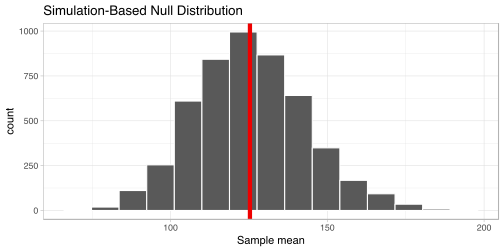
\includegraphics{01-edaR-review_files/figure-latex/unnamed-chunk-9-1.pdf}

\subsubsection{Quantitative variables}\label{quantitative-variables}

\begin{Shaded}
\begin{Highlighting}[]
\KeywordTok{summary}\NormalTok{(HELPrct}\OperatorTok{$}\NormalTok{age)}
\end{Highlighting}
\end{Shaded}

\begin{verbatim}
##    Min. 1st Qu.  Median    Mean 3rd Qu.    Max. 
##   19.00   30.00   35.00   35.65   40.00   60.00
\end{verbatim}

\begin{Shaded}
\begin{Highlighting}[]
\KeywordTok{sd}\NormalTok{(HELPrct}\OperatorTok{$}\NormalTok{age)}
\end{Highlighting}
\end{Shaded}

\begin{verbatim}
## [1] 7.710266
\end{verbatim}

\begin{Shaded}
\begin{Highlighting}[]
\KeywordTok{gf_histogram}\NormalTok{(}\OperatorTok{~}\StringTok{ }\NormalTok{age, }\DataTypeTok{data =}\NormalTok{ HELPrct)}
\KeywordTok{gf_density}\NormalTok{(}\OperatorTok{~}\StringTok{ }\NormalTok{age, }\DataTypeTok{data =}\NormalTok{ HELPrct)}
\end{Highlighting}
\end{Shaded}

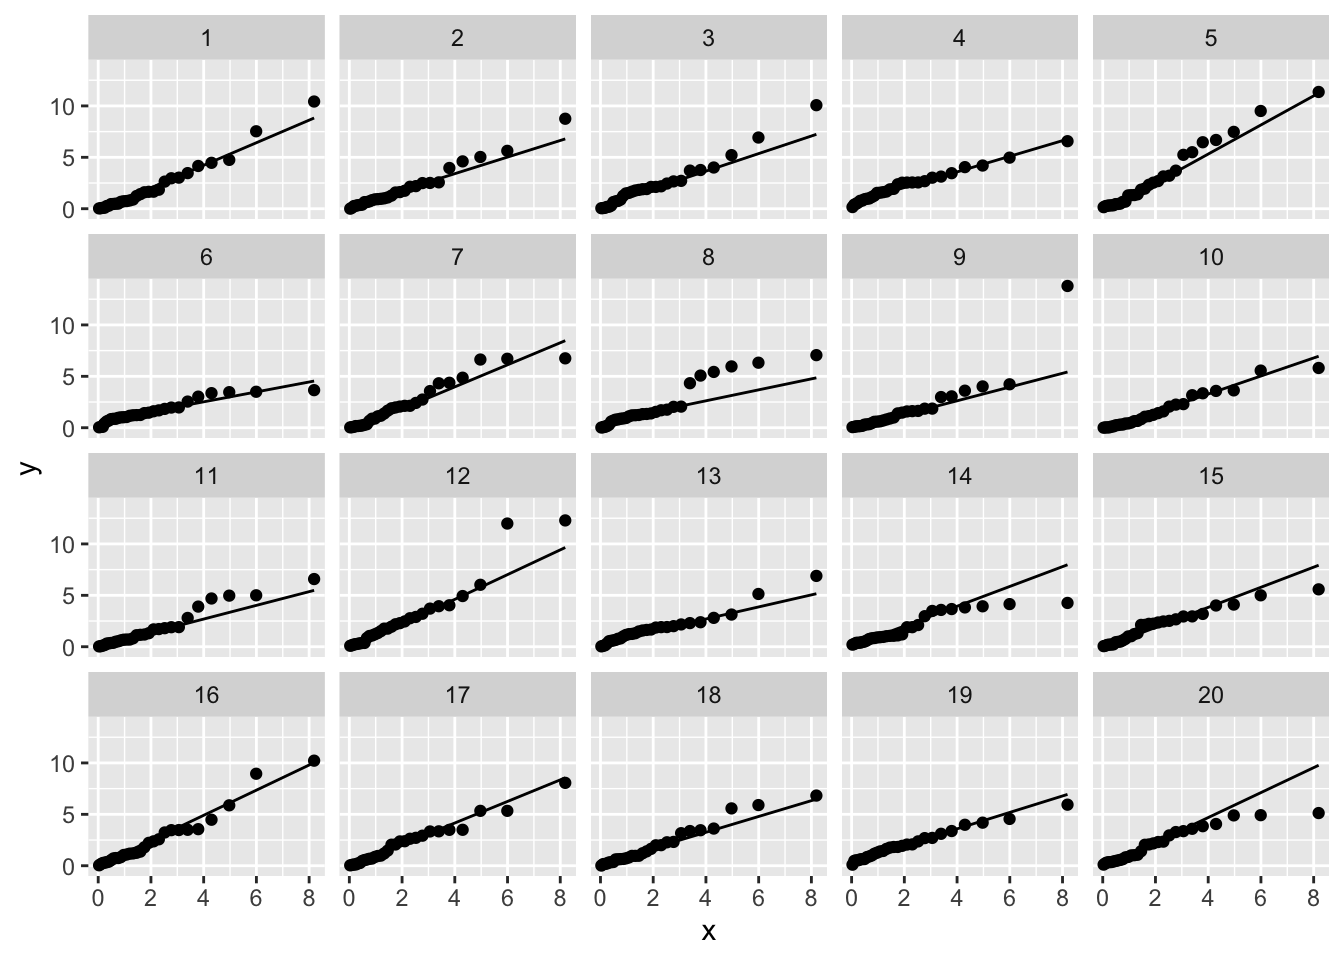
\includegraphics{01-edaR-review_files/figure-latex/unnamed-chunk-12-1.pdf}

\subsection{Bivariate summaries}\label{bivariate-summaries}

\subsubsection{Categorical
vs.~categorical}\label{categorical-vs.categorical}

\begin{Shaded}
\begin{Highlighting}[]
\KeywordTok{table}\NormalTok{(HELPrct}\OperatorTok{$}\NormalTok{sex, HELPrct}\OperatorTok{$}\NormalTok{substance)}
\end{Highlighting}
\end{Shaded}

\begin{verbatim}
##         
##          alcohol cocaine heroin
##   female      36      41     30
##   male       141     111     94
\end{verbatim}

\begin{Shaded}
\begin{Highlighting}[]
\KeywordTok{gf_bar}\NormalTok{( }\OperatorTok{~}\StringTok{ }\NormalTok{substance, }\DataTypeTok{data =}\NormalTok{ HELPrct, }\DataTypeTok{fill =} \OperatorTok{~}\NormalTok{sex)}
\KeywordTok{gf_bar}\NormalTok{( }\OperatorTok{~}\StringTok{ }\NormalTok{substance, }\DataTypeTok{data =}\NormalTok{ HELPrct, }\DataTypeTok{fill =} \OperatorTok{~}\NormalTok{sex, }\DataTypeTok{position =} \KeywordTok{position_dodge}\NormalTok{())}
\KeywordTok{gf_bar}\NormalTok{( }\OperatorTok{~}\StringTok{ }\NormalTok{substance, }\DataTypeTok{data =}\NormalTok{ HELPrct, }\DataTypeTok{fill =} \OperatorTok{~}\NormalTok{sex, }\DataTypeTok{position =} \KeywordTok{position_fill}\NormalTok{())}
\end{Highlighting}
\end{Shaded}

\begin{verbatim}
## Loading required package: viridisLite
\end{verbatim}

\includegraphics{01-edaR-review_files/figure-latex/unnamed-chunk-15-1.pdf}

\subsubsection{Quantitative
vs.~categorical}\label{quantitative-vs.categorical}

\begin{Shaded}
\begin{Highlighting}[]
\CommentTok{# Using dplyr}
\NormalTok{HELPrct }\OperatorTok
\StringTok{  }\KeywordTok{group_by}\NormalTok{(racegrp) }\OperatorTok
\StringTok{  }\KeywordTok{summarize}\NormalTok{(}\DataTypeTok{min =} \KeywordTok{min}\NormalTok{(age),}
            \DataTypeTok{Q1 =} \KeywordTok{quantile}\NormalTok{(age, }\DataTypeTok{prob =}\NormalTok{ .}\DecValTok{25}\NormalTok{),}
            \DataTypeTok{median =} \KeywordTok{median}\NormalTok{(age),}
            \DataTypeTok{Q3 =} \KeywordTok{quantile}\NormalTok{(age, }\DataTypeTok{prob =}\NormalTok{ .}\DecValTok{75}\NormalTok{),}
            \DataTypeTok{max =} \KeywordTok{max}\NormalTok{(age),}
            \DataTypeTok{mean =} \KeywordTok{mean}\NormalTok{(age),}
            \DataTypeTok{sd =} \KeywordTok{sd}\NormalTok{(age),}
            \DataTypeTok{n =} \KeywordTok{length}\NormalTok{(age))}
\end{Highlighting}
\end{Shaded}

\begin{verbatim}
## # A tibble: 4 x 9
##   racegrp    min    Q1 median    Q3   max  mean    sd     n
##   <fct>    <dbl> <dbl>  <dbl> <dbl> <dbl> <dbl> <dbl> <int>
## 1 black       20  31       35  39      60  35.7  7.08   211
## 2 hispanic    21  28.2     32  36.2    55  33.2  7.99    50
## 3 other       22  30       34  40.5    48  35.0  7.66    26
## 4 white       19  30       36  42      58  36.5  8.28   166
\end{verbatim}

\begin{Shaded}
\begin{Highlighting}[]
\KeywordTok{gf_boxplot}\NormalTok{(age }\OperatorTok{~}\StringTok{ }\NormalTok{racegrp, }\DataTypeTok{data =}\NormalTok{ HELPrct)}
\end{Highlighting}
\end{Shaded}

\includegraphics{01-edaR-review_files/figure-latex/unnamed-chunk-16-1.pdf}

\subsubsection{Quantitative
vs.~Quantitative}\label{quantitative-vs.quantitative}

\begin{Shaded}
\begin{Highlighting}[]
\KeywordTok{cor}\NormalTok{(HELPrct}\OperatorTok{$}\NormalTok{i1, HELPrct}\OperatorTok{$}\NormalTok{age)}
\end{Highlighting}
\end{Shaded}

\begin{verbatim}
## [1] 0.2069538
\end{verbatim}

\begin{Shaded}
\begin{Highlighting}[]
\KeywordTok{gf_point}\NormalTok{(i1 }\OperatorTok{~}\StringTok{ }\NormalTok{age, }\DataTypeTok{data =}\NormalTok{ HELPrct)}
\end{Highlighting}
\end{Shaded}

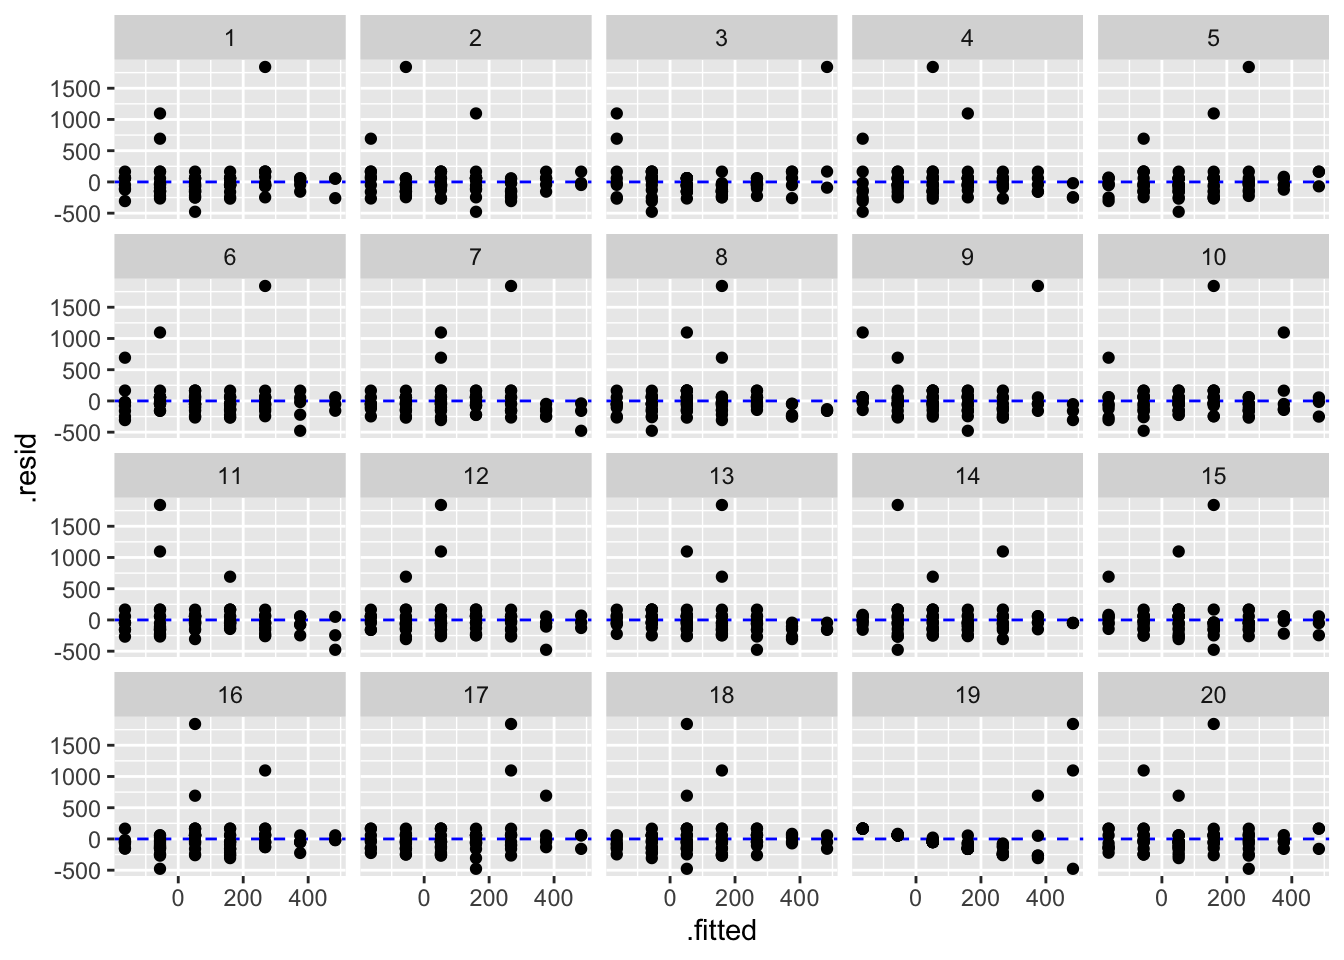
\includegraphics{01-edaR-review_files/figure-latex/unnamed-chunk-17-1.pdf}


\end{document}
